\chapter{Testen und Bewertung}
\label{chap:testen}

Die Umsetzung wurde durch automatisierte Tests, eine heuristische
Evaluation der Oberfläche und die Prüfung ausgewählter
Erfolgskriterien der \acs{WCAG}~2.1 bewertet. Von den vier geprüften Kriterien sind drei erfüllt; der einzige
Verstoß betrifft den Kontrast des Fokusrings.

\section{Automatisierte Tests}
\label{sec:automatisierte_tests}

Die Anwendung enthält 36 Testdateien, die mit \textit{Vitest} und der
\textit{Testing Library} ausgeführt werden und fehlerfrei durchlaufen
(vgl. Abschnitt~\ref{sec:technologieauswahl}). Geprüft werden sowohl
reine Funktionen, etwa die Warenkorbsumme und Datumsaufbereitung, als
auch Komponenten wie Anmelde- und Registrierungsformulare. Ein
besonders relevanter Befund betraf eine fehlerhafte
Datumsformatierung, für die ein Test ergänzt wurde.

End-to-End-Tests mit \textit{Playwright} ergänzen die Modultests durch
die Prüfung vollständiger Nutzerabläufe. Ihre Einrichtung ist noch
nicht abgeschlossen.

\section{Heuristische Evaluation}
\label{sec:heuristische_evaluation}
Die Wahl der heuristischen Evaluation folgt aus den Rahmenbedingungen
der Arbeit. Ein Nutzertest hätte Teilnehmer und eine eigene Auswertung
erfordert und war zeitlich nicht leistbar; die im Unternehmen
vorgesehene Oberflächenprüfung findet erst an einer Vorabfassung und
durch eine andere Person statt. Erforderlich war deshalb ein
Verfahren, das sich von einer Person am eigenen Entwicklungsstand
anwenden lässt und mit den neun Heuristiken zugleich ein Raster über
die gesamte Oberfläche legt (vgl. Tabelle~\ref{tab:heuristiken}).
Die Evaluation folgt dem Verfahren von Nielsen und Molich
\cite{nielsen_molich_heuristic, nielsen_explanatory_power}. Es wurden
nur Befunde mit Ursache im Frontend berücksichtigt. 15 Befunde wurden
nach Nielsens Schweregradskala von null bis vier bewertet
\cite{nielsen_explanatory_power}; sechs weitere Beobachtungen wurden
nach Prüfung des Quellcodes ausgeschlossen.

\begin{table}[H]
\centering
\caption{Befunde der Evaluation}
\label{tab:befunde}
\small
\begin{tabular}{|l|p{4.6cm}|p{3.1cm}|c|l|}
\hline
\textbf{Nr} & \textbf{Befund} & \textbf{Heuristik} & \textbf{Grad} & \textbf{Status} \\
\hline
B1 & Anbieterbereich bei laufendem Antrag & Systemstatus & 3 & behoben \\
\hline
B2 & Hinterlegte Meldung wird nicht erreicht & Fehlerbehebung & 2 & behoben \\
\hline
B3 & Meldung benennt andere Regel & Fehlerbehebung & 2 & behoben \\
\hline
B4 & Storno nach Fristablauf & Fehlervermeidung & 3 & behoben \\
\hline
B5 & Überlappende Buchungszeiten & Fehlervermeidung & 2 & behoben \\
\hline
B6 & Rollenbereiche ohne Übersetzung & Reale Welt & 3 & behoben \\
\hline
B7 & Telefonfeld nicht als optional erkennbar & Wiedererkennung & 1 & geklärt \\
\hline
B8 & Erfolgsseite bietet beide Übersichten & Minimalismus & 2 & behoben \\
\hline
B9 & Interner Bezeichner in der Oberfläche & Reale Welt & 2 & behoben \\
\hline
B10 & Sprachwahl nicht ans Backend übertragen & Reale Welt & 3 & behoben \\
\hline
B11 & Positionsstatus widerspricht der Buchung & Systemstatus & 2 & behoben \\
\hline
B12 & Zwei gleichrangige Rückwege & Konsistenz & 2 & behoben \\
\hline
B13 & Englische Abkürzung in der Oberfläche & Reale Welt & 1 & behoben \\
\hline
B14 & Umbuchen auf Deutsch unbenutzbar & Fehlervermeidung & \textbf{4} & behoben \\
\hline
B15 & Eigenes Angebot buch- und kaufbar & Fehlervermeidung & 3 & behoben \\
\hline
\end{tabular}
\end{table}

Zusätzlich wurden drei technische Beobachtungen ohne
Usability-Schweregrad festgestellt: die nicht getrennte
Echtzeitverbindung beim Abmelden, wachsende Kanalabonnements und feste
Rückfallwerte im Quelltext. Die ersten beiden werden in
Kapitel~\ref{chap:fazit} aufgegriffen.

Auffällig ist die Häufung sprachbezogener Befunde. Vier der 15
Befunde betreffen die Übereinstimmung mit der realen Welt; zusammen
mit B14 betrifft damit etwa ein Drittel der Befunde die
Mehrsprachigkeit. B14 zeigt dies besonders deutlich: Ein Datum wurde
auf Deutsch für die Oberfläche formatiert und anschließend in diesem
Format an die Schnittstelle übergeben. Auf Englisch funktionierte dies
zufällig. Das Mehrsprachigkeitskonzept ist damit grundsätzlich
geeignet, wurde jedoch nicht in allen Bereichen konsequent geprüft.

\section{Normbezogene Prüfung}
\label{sec:normbezogene_pruefung}

Während die Heuristiken eine qualitative Bewertung ermöglichen, legt
die \acs{WCAG} konkrete Schwellenwerte fest. Geprüft wurden vier
Erfolgskriterien aus Abschnitt~\ref{subsec:barrierefreiheit}
\cite{wcag21}.

\begin{table}[H]
\centering
\caption{Prüfung gegen vier Erfolgskriterien der WCAG 2.1}
\label{tab:wcag_pruefung}
\begin{tabular}{|l|p{6.2cm}|p{3.4cm}|}
\hline
\textbf{Kriterium} & \textbf{Inhalt} & \textbf{Ergebnis} \\
\hline
1.4.3 & Kontrast von Text, 4,5:1 & erfüllt \\
\hline
1.4.11 & Kontrast von Bedienelementen, 3:1 & nicht erfüllt \\
\hline
1.4.10 & Nutzbar bis 320~px ohne waagerechtes Scrollen & erfüllt \\
\hline
2.1.1 & Alle Funktionen über die Tastatur erreichbar & erfüllt \\
\hline
\end{tabular}
\end{table}

Für Kriterium~1.4.10 wurden neun Hauptansichten bei 320~px Breite
geprüft. Es trat kein waagerechtes Scrollen auf und kein Inhalt blieb
unerreichbar. Abbildung~\ref{fig:reflow_320} zeigt die anspruchsvollste
Ansicht mit Kalender, Zeitzone und Zeitfenstern.

\begin{figure}[htbp]
\centering
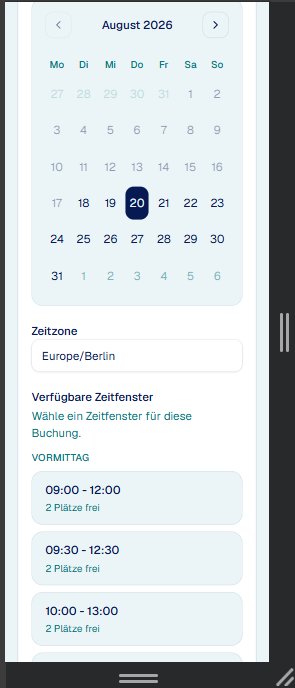
\includegraphics[width=0.25\textwidth]{Bilder/screenshot_reflow_320.png}
\caption{Terminauswahl bei einer Anzeigebreite von 320~px}
\label{fig:reflow_320}
\end{figure}

Kriterium~2.1.1 wurde mit \texttt{Tab}, \texttt{Umschalt+Tab},
\texttt{Enter}, \texttt{Leertaste} und \texttt{Esc} geprüft. Die
untersuchten Bereiche waren vollständig bedienbar. Beim Schließen des
Anmeldedialogs kehrt der Fokus jedoch nicht zur auslösenden
Schaltfläche zurück; dies betrifft Kriterium~2.4.3 und wurde nicht
bewertet.

Die Farbwerte des Designsystems sind paarweise definiert, sodass sich
jedes Verhältnis unmittelbar bestimmen lässt (vgl.
Abschnitt~\ref{subsec:designsystem}). Der Fließtext erreicht auf einer
Karte 16,5:1 und auf dem Seitenhintergrund 14,8:1, der gedämpfte Text
5,3:1 auf der Karte und 4,7:1 auf dem Seitenhintergrund. Sämtliche
Textpaarungen erfüllen damit Kriterium~1.4.3.

Beim Fokusring fallen Entwurf und Darstellung auseinander. Der
hinterlegte Wert ergäbe gegenüber einer Karte 3,6:1 und damit mehr als
die geforderten 3:1. Tatsächlich wird der Ring jedoch über eine
globale Regel mit halber Deckkraft gegen den Untergrund gemischt,
sodass nur 1,8:1 verbleiben. Er ist damit vorhanden und
sichtbar, aber nicht normkonform, und Kriterium~1.4.11 ist nicht
erfüllt. Diese Unterscheidung ist der eigentliche Ertrag der Messung:
Ob eine Anzeige wahrnehmbar ist, lässt sich betrachten; ob sie einen
Schwellenwert erreicht, nicht, und ein Blick auf die Farbwerte allein
genügt dafür ebenfalls nicht.

\section{Grenzen des Verfahrens}
\label{sec:grenzen_verfahren}

Die Evaluation wurde von einem einzelnen Evaluator durchgeführt und
stellt daher keine vollständige Erhebung dar
\cite{nielsen_molich_heuristic}. Da Evaluator und Entwickler dieselbe
Person sind, besteht zudem ein Risiko für eine unbewusste Orientierung
am vorgesehenen Nutzungspfad. Die heuristische Evaluation ersetzt
keinen Nutzertest. Außerdem wurden nur vier Erfolgskriterien der
Stufe~AA geprüft, weshalb keine vollständige WCAG-Konformität
abgeleitet werden kann.

\section{Bewertung der Ergebnisse}
\label{sec:bewertung}

Die Ergebnisse werden den nicht-funktionalen Anforderungen aus
Tabelle~\ref{tab:nichtfunktionale-anforderungen} gegenübergestellt.

Responsivität und Barrierefreiheit wurden anhand der relevanten
\acs{WCAG}-Kriterien geprüft. Die Kriterien~1.4.10 (Responsivität),
2.1.1 (Tastaturbedienung) und 1.4.3 (Textkontrast) sind erfüllt.
Nicht erfüllt ist Kriterium~1.4.11, da eine globale Regel den
Fokusring mit halber Deckkraft darstellt und er dadurch den
geforderten Wert unterschreitet. Die Korrektur betrifft lediglich
eine globale Regel.

Für die Performance ist der Programmcode auf 102 Dateien aufgeteilt,
von denen beim ersten Aufruf nur ein Teil übertragen wird. Die größte
Datei umfasst 230~kB und bleibt damit unter der vom Build-Werkzeug
genannten Schwelle von 500~kB.
Die Antwortzeiten wurden am gebauten Stand gemessen, jeweils vom Klick
bis zum nächsten Bildaufbau. Die Formularvalidierung, die ohne Anfrage
an das Backend auskommt, lag über vier Durchläufe zwischen 14 und
33~Millisekunden und damit unterhalb der geforderten 0,1~Sekunden. Der
Wechsel von der Produktliste auf eine Produktseite einschließlich des
Nachladens des zugehörigen Codestücks lag bei 10~Millisekunden und
damit unterhalb der geforderten Sekunde. Vorgänge mit Anfrage an das
Backend reagierten innerhalb von 17 bis 19~Millisekunden mit einem
Ladezustand; ihre Gesamtdauer hängt von der Antwortzeit der
Schnittstelle ab und ist nach Abschnitt~\ref{sec:abgrenzung} nicht
Gegenstand dieser Arbeit.

Die Sicherheit wurde nicht eigenständig geprüft. Die heuristische
Evaluation zeigte jedoch einen Befund (B1) beim rollenbasierten
Seitenschutz. Da die eigentliche Zugriffskontrolle serverseitig
erfolgt, dient der Frontend-Schutz hauptsächlich der Benutzerführung.

Die Wartbarkeit wurde anhand der Projektstruktur bewertet. Die
16 Funktionsbereiche unter \texttt{features/} folgen demselben Schema
aus Datenzugriff, Komponenten, Hooks, Seiten, Schemata und Typen,
jeweils beschränkt auf die benötigten Bestandteile (vgl.
Abschnitt~\ref{subsec:komponentenarchitektur}). Damit wurde die
geplante Architektur im gesamten Quellstand umgesetzt. Aussagen über
den zukünftigen Änderungsaufwand sind daraus jedoch nicht ableitbar.